\documentclass{article}
\usepackage{graphicx} % Required for inserting images
\usepackage{biblatex}
\addbibresource{references.bib}
% \usepackage[sortcites=true,sorting=nyt,backend=biber]{biblatex}
\usepackage{hyperref}
\usepackage{amsmath}
\usepackage{amssymb}
\usepackage{caption}
\usepackage{subcaption}

\bibliography{references}

\title{Evolving Training Sets for Peptide Discrimination via Evolutionary Algorithms}
\author{Loek Gerrits (s1032343), Evangelos Spithas (s1125593), Bart van Nimwegen}
\date{\today}

\begin{document} 

\maketitle

\section{Introduction}

\subsection{Background}

In human bodies, the immune system is responsible for detecting pathogens and exterminating them. 
One of the tools at its disposal, is the T cells. T cells grow in the thymus, and each one is responsible for
identifying and attacking specific cells. However, that means that it is possible for healthy cells to be
attacked as well. In order to mitigate this, human cells are presented to the T cells, and the T cells that attack them 
are eliminated. This process is called Negative Selection (NS). In practice, the amount of possible cells is very large, and as a result only a sub-set of self peptides are presented
in the T cells. 

\subsection{Relevance}
Negative Selection algorithms have a number of  applications in both biological algorithms and computer algorithms.
Understanding Negative selection for biology can improve our understanding of, for example how the immune system handles
negative cells, which can prevent certain diseases. For computer algorithms, Artificial Immune Systems (AIS) are systems
that draw inspiration from the human immune system, similarly to how Neural Networks (NNs) are inspired by the human 
nervous system, Negative Selection (NS) Algorithms are also part of these AIS, and are often used for anomaly detection 
or classification.

For both the biological algorithms and computer algorithms, the effectiveness of the NS algorithm heavily depends
on the quality of the training data, especially the subset of self-peptides that is used to eliminate T-cells that
could otherwise cause harm . Since using all the self-peptides is not really possible,
as the number of self-peptides is too big it would be too expensive to process all of them.

Therefore being able to find the optimal subset to use for the NS algorithm is crucial to improve the accuracy of the 
NS algorithm.  

\subsection{Problem description}

In this project, we would like to explore how we can find this optimal subsets to train an NS algorithm for peptide 
selection. We will do this using 3 different methods, randomly sampling a subset, using a greedy algorithm and an 
Evolutionary Algorithm (EA) to produce them. Afterwards, we will train the negative selection algorithm with each one of
them, and evaluate its performance against different sets of harmful peptides, such as HIV and ebola cells. Additionally,
we will be performing the Negative Selection on different language such as Xhosa and Tagalog and check if we get better 
results for using different sets of peptides, generated by the three algorithms. 

\subsection{Related work}
This project is an extension to the paper by Wortel et al \cite{wortel2020t}, They developed a greedy algorithm to 
approximate an optimal training set for NSA training, and found that the "artificial immune system" performed better in 
terms of generalization and discrimination using such optimized training sets. We want to verify those findings by 
comparing this greedy algorithm using a randomly selected training set and a training set created by an evolutionary 
algorithm.\\

In the paper by Wilde et al. \cite{wilde2020evolutionary} they propose a solution on how evolutionary algorithms can 
have a positive impact on optimizing training sets for classification problems.
We hope to include and apply those findings when we are implementing our evolutionary algorithm to create an 
optimized training set.

\section{Methodology}
\subsection{Datasets} \label{datasets}
This study first tried to deal with the easier problem of discriminating two different languages, and later on we 
consider the harder problem of distinguishing human peptides from foreign ones. Therefore, the datasets used in our 
experiments consist of two parts: 1) languages and 2) peptides. Each consists of a training set containing all the self 
peptides for negative selection, and test datasets containing foreign peptides and one with self peptides. In all our 
experiments, we set the length of short strings and peptides (from now on, for the sake of brevity, we will also refer 
to the strings in the language datasets as peptides, as they are functionally not different) to $n$ to $n=6$.

For the language datasets, we first defined a common alphabet of size of 27 which includes an additional '$\_$' to 
signify spaces in the text and the 26 letters of the English alphabet.
All texts were preprocessed such that every character not in the alphabet was replaced with a 
'$\$', and, as an extra pass, there could only be a single '$\$' back-to-back. After that, we generated a training 
dataset ($n=189718$) and a test set of strings of a length of 6 based on the novel 'Moby Dick' by Herman Melville.
Then, test sets of foreign peptides were generated based on the first few chapters of The Ghospel of Matthew from the 
Bible for the following languages: Hiligaynon, Latin, Middle-English, Plautdietsch, Tagalog and Xhosa. 
The test sets were all $2000$ peptides long.

For the experiments with peptides, we used the various peptide datasets that were used by \textcite{wortel2020t} in 
their experiments found in their GitHub (\url{https://github.com/ingewortel/negative-selection-2020}). From this, we 
used the human peptides as the training ($n=262000$) and test sets of self peptides ($n=1216$), and peptides of the
following diseases were defined as foreign peptides and used as test sets of various sizes: HIV, hepatitis B, and ebola. 
These peptide datasets used an alphabet of amino acids of length 20 (ACDEFGHIKLMNPQRSTVWY) as opposed to 28 from the languages part.

\subsection{Optimizers} \label{optimizers}

In order to create more effective training dataset of self peptides for negative selection, we implemented two 
optimizers: 1) a greedy algorithm and 2) the evolutionary algorithm. These strategies try to select subsets that 
maximize the information of the training data.

\subsubsection{Greedy Algorithm}

The greedy algorithm iteratively builds a data set by greedily selecting a) the peptide that matches with the greatest 
umber of motifs and b) removing its matching motifs from the motifs set until there are no motifs left. A peptide 
matches with a motif when the number of consecutive AAs at their respective positions is equal to or greater than 
threshold $t$. For both parts, we used $t=3$ and generated all possible motif combination with length $n$ and the 
current alphabet, resulting in $27^6$ motifs for the language part and $20^6$ motifs for the peptide part.

Because the greedy algorithm has a high complexity (in every iteration, each peptide needs to be compared to all 
current motifs), computing the fully optimized dataset using all human peptides and all possible motifs was infeasible.
Therefore, this study randomly sampled only $1\%$ of all motifs to reduce the runtime of the experiments, and $4\%$ of 
the self peptides. The greedily optimized dataset for each part also determined the size of the other generated datasets 
(3574 for languages, and 6125 for peptides). We did this because we wanted the comparisons between the other 
(random and evolved) resulting datasets to be consistent.

\subsubsection{Greedy Algorithm}

The greedy algorithm optimizes ...

Because the greedy algorithm has a high complexity, computing the fully optimized dataset using all human peptides and
all possible motifs was infeasible. Therefore, this study limited the number of peptides and motifs.


\subsubsection{Evolutionary Algorithm} 

\paragraph{AA composition}



\paragraph{AA frequency}

\paragraph{Exchangeability}


\subsection{Negative Selection}
In order to run the negative selection experiments we will use the jar that is provided by \url{https://johannes-textor.name/negativeselection.html}.
The training of the algorithm will take place with the three training sets as described in section \ref{datasets}.
All elements of each dataset have a fixed length of 6, and we will evaluate the effectiveness of the NS algorithm by 
experimenting  with a variable length of contiguous selectors, ranging between 1 and 6. 

For each peptide in the test datasets, the NS algorithm can return either the number of patterns in the repertoire that 
match it, or the normalised value $log_2(1 + x)$, where $x$ is the number of matching patterns. We will use this 
normalised value here, as the number of selectors can be unwieldy to work with. Afterwards, we can classify each peptide 
as anomalous or self peptide, if its score exceeds the value r.
% jar counts all matching selectors so we do log to get better anomaly scores

\subsection{Experimental design}
We set the following experimental setup to test our methods. We first generated three subsets of the english dataset 
from the text of Mobby Dick, with the methods described in section \ref{optimizers}, which we will use as the self set of 
the negative selection algorithm. The datasets have a size 3574. This was the size of the dataset returned by the greedy 
algorithm and was then used as the target size of the datasets of the other methods.

As test sets, we used an english dataset with 2000 english tokens, which were obtained by random excerpts from The Bible (\url{https://www.wordproject.org/bibles/index.htm}).
We also repeated the same method to obtain test datasets in the following languages: Hiligaynon, Latin, Middle English, 
Plautdietsch, Tagalog and Xhosa. The NS algorithm was run for each language, and after classifying the data, we 
estimated the receiver operating characteristic curve (AUC) to quantify how well our estimated datasets can optimise 
the NS algorithm.

Lastly, we repeated the same experiments but with actual peptide data. For that we used a subset of human peptides with 
size 1216, as well peptides of the following diseases: HIV, hepatitis B, and ebola, as obtained by \url{https://github.com/ingewortel/negative-selection-2020}



\section{Results}
\subsection{Language Discrimination}
In Figures \ref{fig:langs_random}, \ref{fig:langs_greedy}, \ref{fig:langs_ea}, we see the Receiver Operating 
Characteristic (ROC) curves and AUC scores of the NS algorithm, for different r values for discrimination between
english and each other language. First of all, we can observe that for $r=1$, the algorithm performs very poorly. That 
is to be expected, as for that value we look for contiguous patterns of length $1$, which are very small to carry any 
important information. As the value of r increases, so does the AUC, until it reaches $r=4$, as it then starts to 
decrease again, very steeply from $5$ to $6$, which potentially shows that we have a lot of false positives. The best 
results are achieved for either $r=3$ or $r=4$.

If we now compare the performance for each language, we can observe that for Middle English, for all the different self 
datasets, the results are poor. This happens because Middle English is very similar to modern English, without enough 
distinctions for the NSA to pick up. The more different the language gets from English, the better results we have, 
with Xhosa, having the best AUC values.

Lastly, we shall evaluate the performance between each different self dataset we have created. Overall, all the datasets 
achieve similar results, without big differences. This means that they all carry meaningful information to 
discriminate the languages. If we look closely, we will see that when using the dataset generated from the evolutionary 
algorithm, we achieve the best performance in Hiligaynon, Latin, Tagalog and Xhosa. The random self dataset achieves the 
best results for Plautdietsch, while the greedy self dataset performs the best with Middle English. As we can see, we 
do not achieve significant gains from the different datasets, however the evolutionary datasets seems promising as it is 
always the best or second best.

For the evolutionary algorithm, we can also look at how the fitness progresses over the generations. In Figure 
\ref{fig:ea_fit_over_gens}, we plot the average and the best fitness for each generation. As we can see, fitness 
converges very fast in the beginning and then it seems to stabilize. This might signal that we could have used more 
individual populations than we did, in order to achieve even more improved results, but this was not feasible due to 
time constraints, since the runtime scales linearly with the size of the population. 

\begin{figure}[ht]
    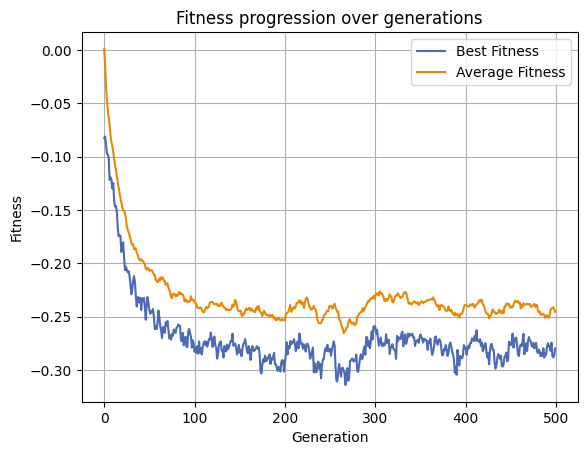
\includegraphics[width=0.75\textwidth]{images/fitness_over_gens.jpeg}
    \caption{Best and Average fitness of the evolutionary algorithm over generations}
    \label{fig:ea_fit_over_gens}
\end{figure}

\subsection{Foreign Peptide Detection}
Next we will have a look at the results for foreign peptide detection. In Figures \ref{fig:pept_rnd}, \ref{fig:pept_grd}, 
\ref{fig:pept_ea},  we see the ROC curves and AUC scores of the NS algorithm, for different r values for discrimination 
between self peptides and Ebola, Hepatitis-B and HIV peptides. As we can observe, the results are rather poor for all 
the differently created self datasets. This indicates that the discrimination of foreign and self peptides is a rather 
difficult problem, most probably because of the similarities between peptides, unlike the more complex structure of 
languages. It is worth noting however, that we still observe a small bump in the AUC scores for $r$ values of $3$ and 
$4$, like before.

\section{Discussion}
In the Results section we observed that the performance for the peptide detection was unfortunately very poor. This stems
from the fact that the foreign peptides have patterns too similar to the human peptides. On the other hand, in the 
languages problem we saw that the NS algorithm performed relatively well, except Middle English, which are also very 
similar to modern English. 

In the future we can explore improvements in the greedy and evolutionary algorithms we used to generate the optimised 
self peptide datasets. With regard to the evolutionary algorithm, we can experiment with different weights for the
features we used to define the fitness function. As we were not able to carry out extensive experiments for them, it is 
possible that there is a better solution that was not explored as part of this work. Moreover, we did not explore any
of the parameters of the evolutionary algorithm, where, for different values we could potentially achieve better
results. Also, the size og the population is currently hardcoded. In the future we could use an implementation with an
adaptive population size that can lead to potentially more optimal solutions.

Furthermore, for the greedy algorithm, we can benefit from increased computational resources, since we were 
forced to only used small subsets of out full datasets. Lastly, potential future work can entail exploring more languages to have a more diverse set of data, as well as pondering 
on more advanced problems, such as distinction between human and LLM generated text.

\section{Conclusion}
In this work, we examined how we can improve the effectiveness of natural selection algorithms, by sampling the training
datasets with three different ways, randomly, with a greedy and with an evolutionary algorithm. We performed two sets of
experiments, one for language discrimination and one for foreign peptide detection. As we saw, creating the training
dataset with the greedy and evolutionary algorithms can improve the NS algorithms, however, due to the limitations we
faced, we could not achieve significant improvements.

The optimal values of $r$ were proven to be $3$ and $4$, while we saw very good results for the discrimination of Xhosa,
followed by the other languages that are not close to English. The problem of discriminating English from Middle English
was proven particularly difficult, same with the detection of foreign peptides, as the structure of all these datasets
are very similar.

There can be many potential gains from NS algorithms and the improvements that we can offer with optimized training
datasets. However, due to the limitations we faced in this work we could not achieve the desired results. Hopefully, 
future work in this field can be proven more fruitful and achieve better results.


\printbibliography

\appendix
\section{Figures}

\begin{figure}[ht]
    \begin{subfigure}[t]{\linewidth}
        \centering
        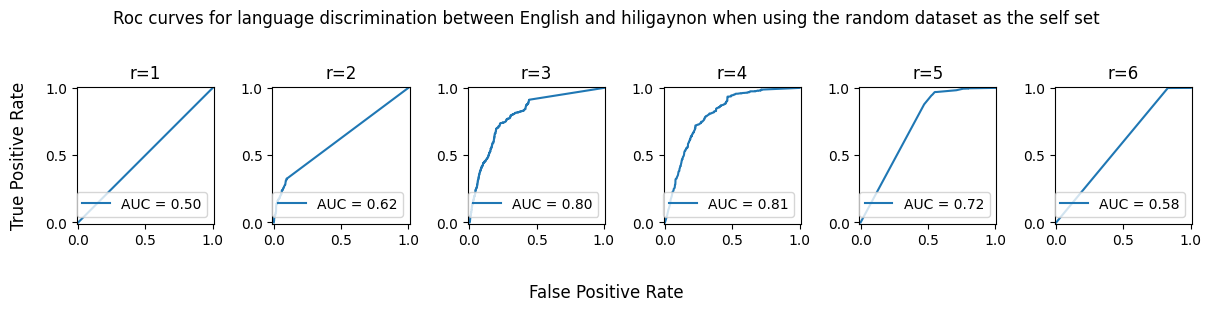
\includegraphics[width=\linewidth]{images/english_hiligayon_random.png}
        \label{fig:eng_hil_rnd}
    \end{subfigure}
    \\
    \begin{subfigure}[t]{\linewidth}
        \centering
        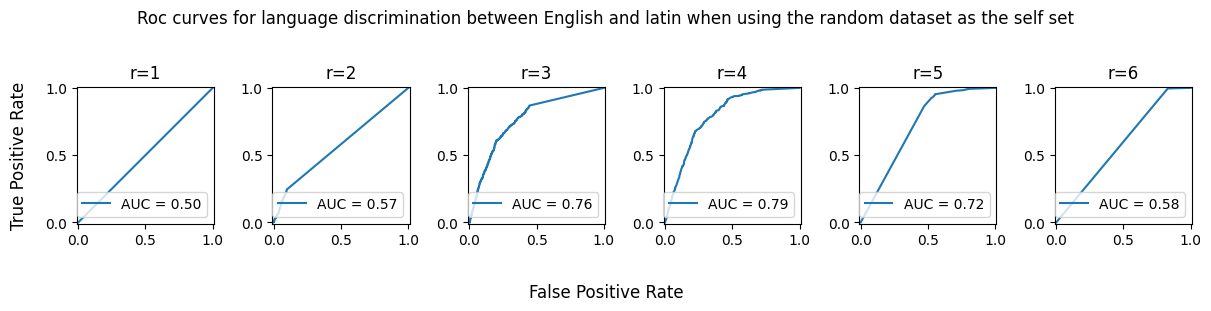
\includegraphics[width=\linewidth]{images/english_latin_random.png}
        \label{fig:eng_lat_rnd}
    \end{subfigure}
    \\
    \begin{subfigure}[t]{\linewidth}
        \centering
        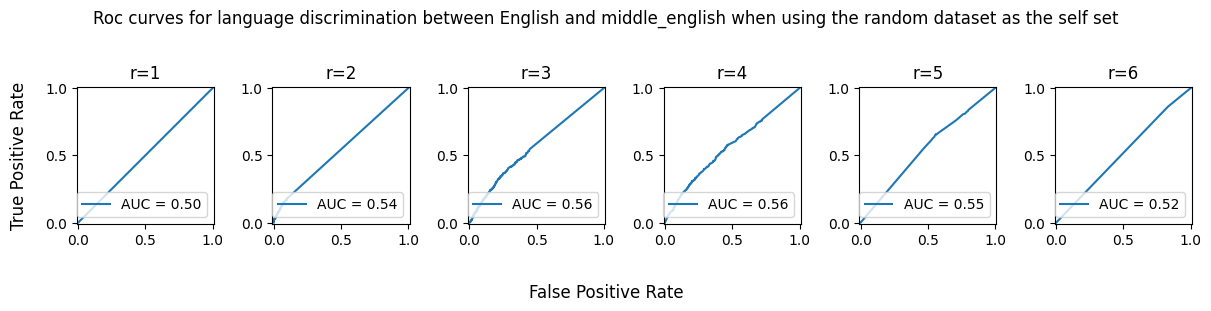
\includegraphics[width=\linewidth]{images/english_middle_neglish_random.png}
        \label{fig:eng_mid_eng_rnd}
    \end{subfigure}
    \\
    \begin{subfigure}[t]{\linewidth}
        \centering
        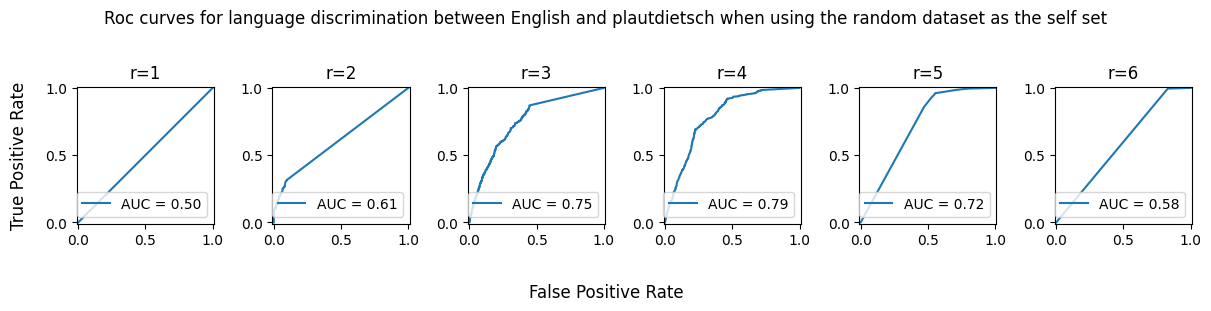
\includegraphics[width=\linewidth]{images/english_platudietsch_random.png}
        \label{fig:eng_mid_pla_rnd}
    \end{subfigure}
    \\
    \begin{subfigure}[t]{\linewidth}
        \centering
        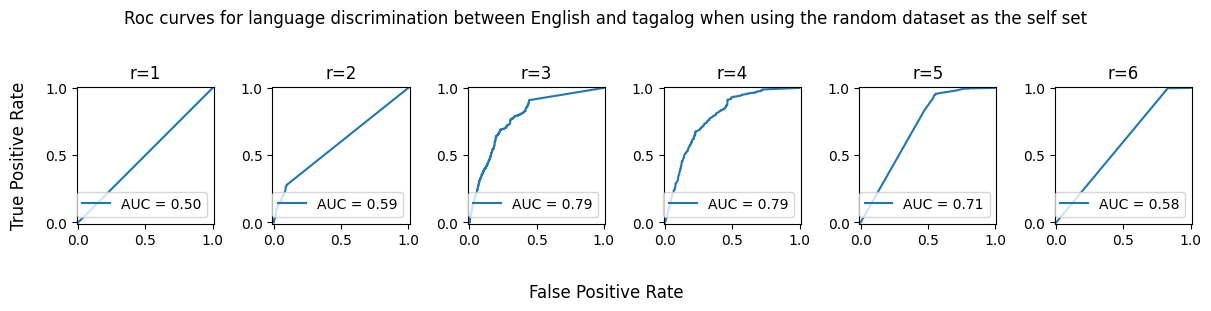
\includegraphics[width=\linewidth]{images/english_tagalog_random.png}
        \label{fig:eng_mid_tag_rnd}
    \end{subfigure}
        \\
    \begin{subfigure}[t]{\linewidth}
        \centering
        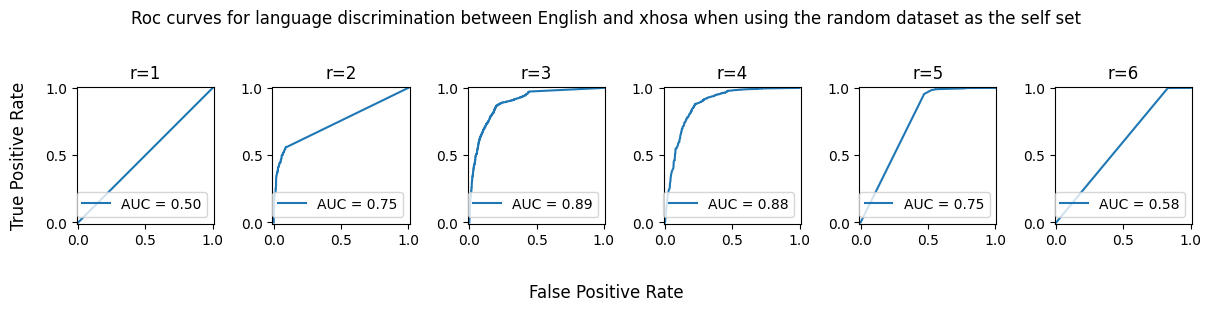
\includegraphics[width=\linewidth]{images/english_xhosa_random.png}
        \label{fig:eng_xho_rnd}
    \end{subfigure}
    
    \caption{ROC curves for language Discrimination between English and each other language, when using the random dataset for the self set}
    \label{fig:langs_random}
\end{figure}

\begin{figure}[ht]
    \begin{subfigure}[t]{\linewidth}
        \centering
        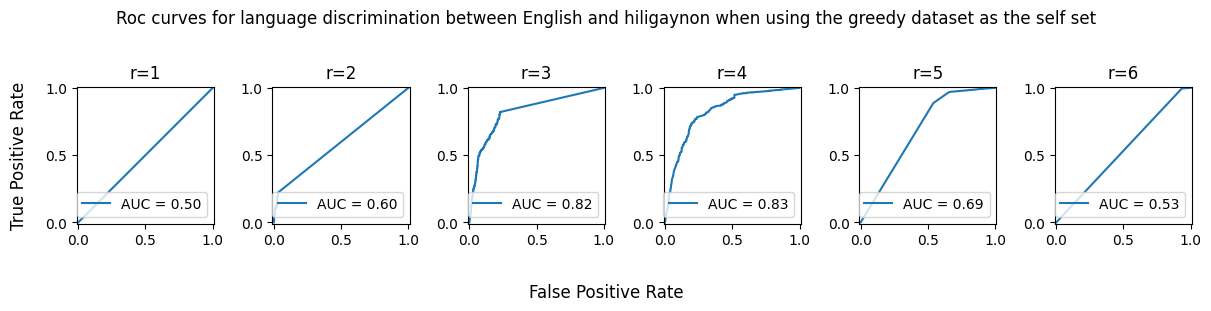
\includegraphics[width=\linewidth]{images/english_hiligayon_greedy.png}
        \label{fig:eng_hil_grd}
    \end{subfigure}
    \\
    \begin{subfigure}[t]{\linewidth}
        \centering
        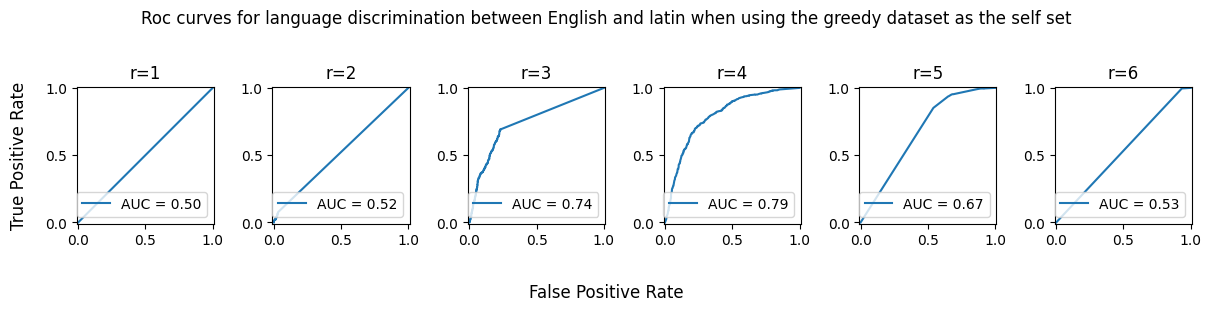
\includegraphics[width=\linewidth]{images/english_latin_greedy.png}
        \label{fig:eng_lat_grd}
    \end{subfigure}
    \\
    \begin{subfigure}[t]{\linewidth}
        \centering
        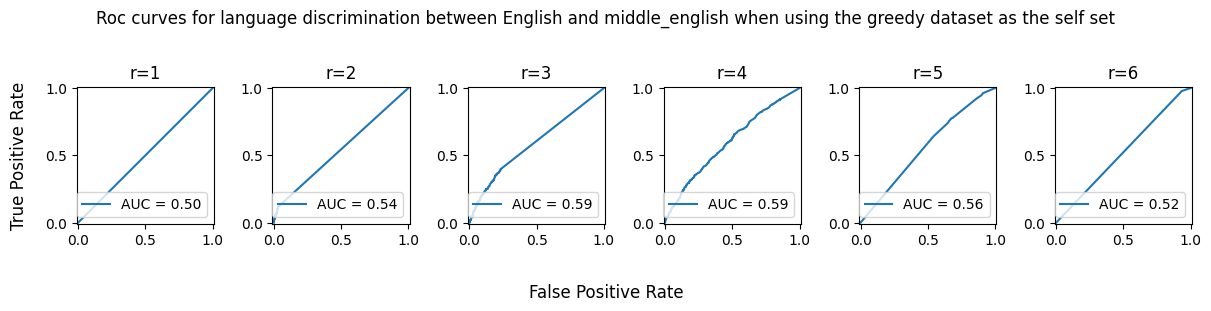
\includegraphics[width=\linewidth]{images/english_middle_neglish_greedy.png}
        \label{fig:eng_mid_eng_grd}
    \end{subfigure}
    \\
    \begin{subfigure}[t]{\linewidth}
        \centering
        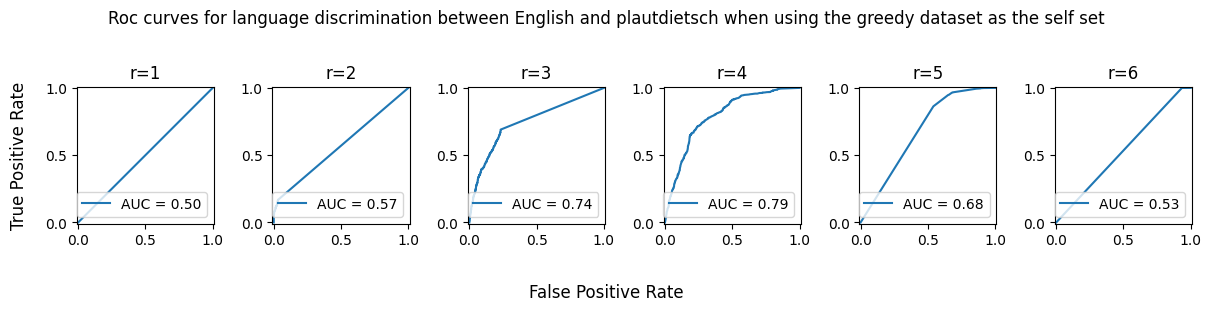
\includegraphics[width=\linewidth]{images/english_platudietsch_greedy.png}
        \label{fig:eng_mid_pla_grd}
    \end{subfigure}
    \\
    \begin{subfigure}[t]{\linewidth}
        \centering
        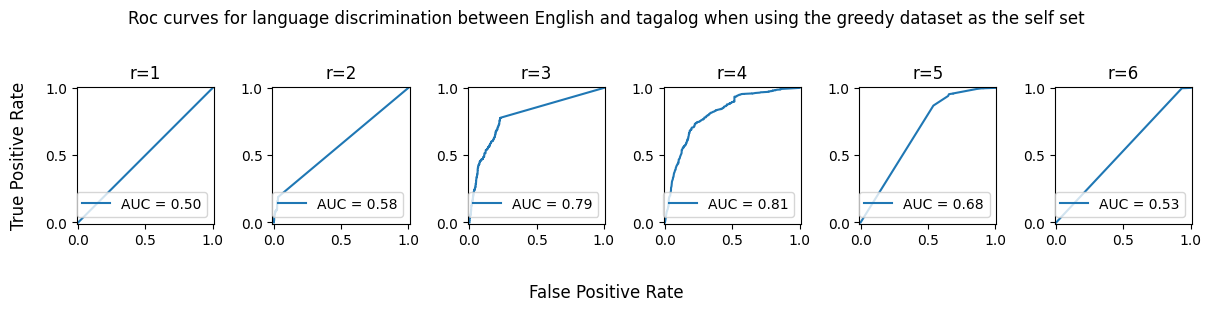
\includegraphics[width=\linewidth]{images/english_tagalog_greedy.png}
        \label{fig:eng_mid_tag_grd}
    \end{subfigure}
        \\
    \begin{subfigure}[t]{\linewidth}
        \centering
        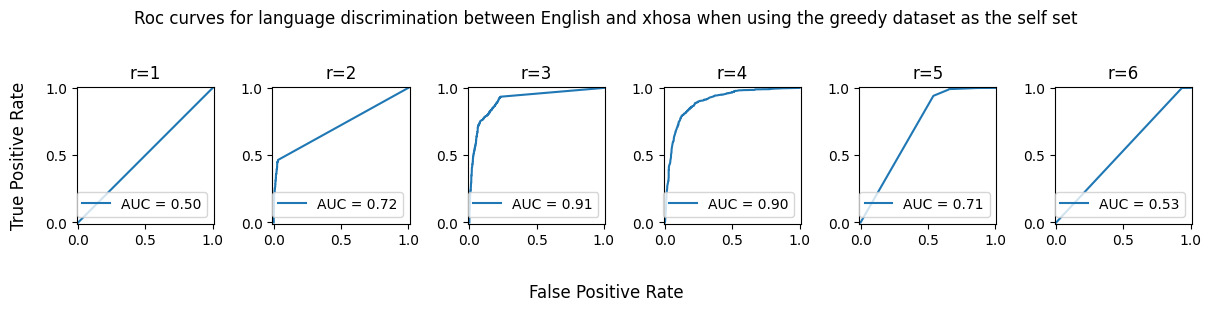
\includegraphics[width=\linewidth]{images/english_xhosa_greedy.png}
        \label{fig:eng_xho_grd}
    \end{subfigure}
    
    \caption{ROC curves for language Discrimination between English and each other language, when using the greedy dataset for the self set}
    \label{fig:langs_greedy}
\end{figure}

\begin{figure}[ht]
    \begin{subfigure}[t]{\linewidth}
        \centering
        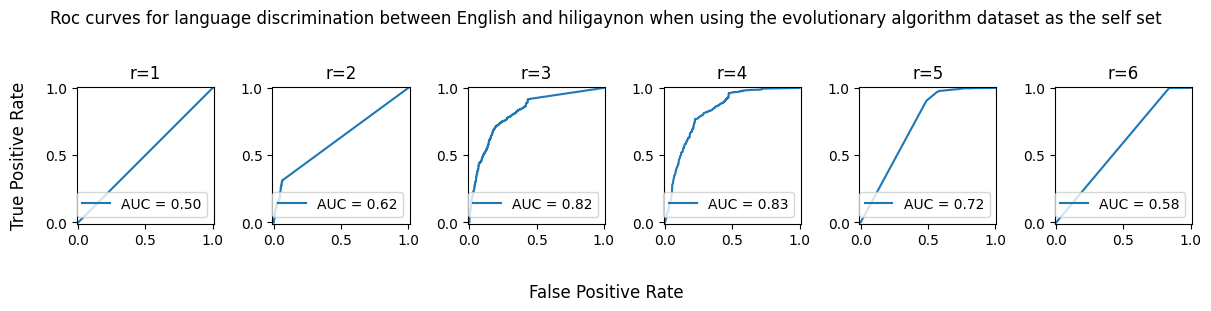
\includegraphics[width=\linewidth]{images/english_hiligayon_ea.png}
        \label{fig:eng_hil_ea}
    \end{subfigure}
    \\
    \begin{subfigure}[t]{\linewidth}
        \centering
        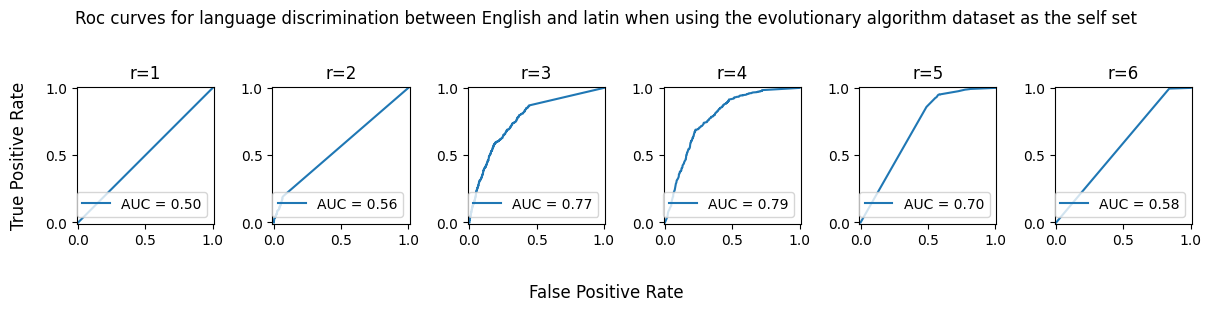
\includegraphics[width=\linewidth]{images/english_latin_ea.png}
        \label{fig:eng_lat_ea}
    \end{subfigure}
    \\
    \begin{subfigure}[t]{\linewidth}
        \centering
        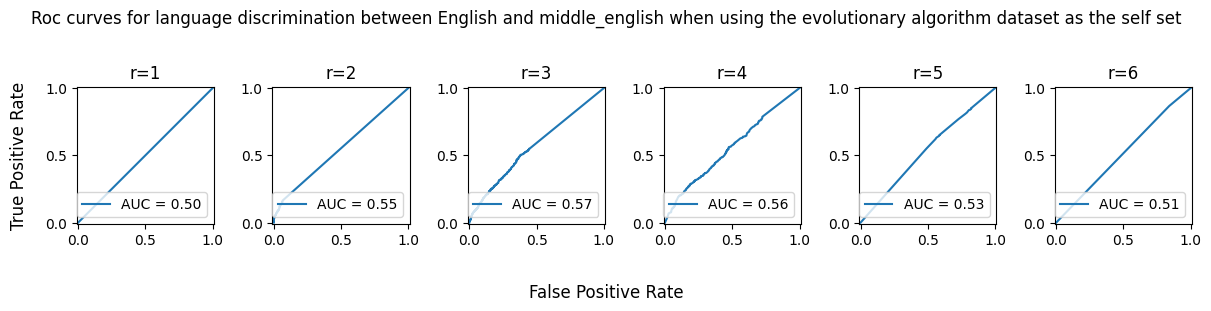
\includegraphics[width=\linewidth]{images/english_middle_neglish_ea.png}
        \label{fig:eng_mid_eng_ea}
    \end{subfigure}
    \\
    \begin{subfigure}[t]{\linewidth}
        \centering
        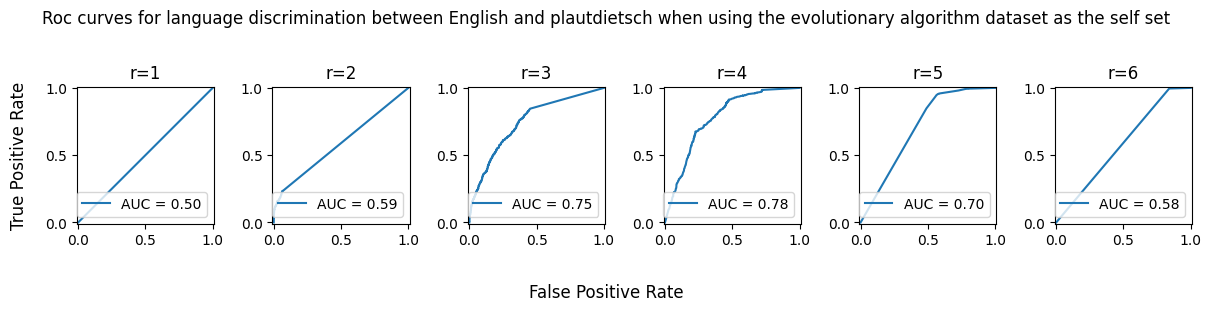
\includegraphics[width=\linewidth]{images/english_platudietsch_ea.png}
        \label{fig:eng_mid_pla_ea}
    \end{subfigure}
    \\
    \begin{subfigure}[t]{\linewidth}
        \centering
        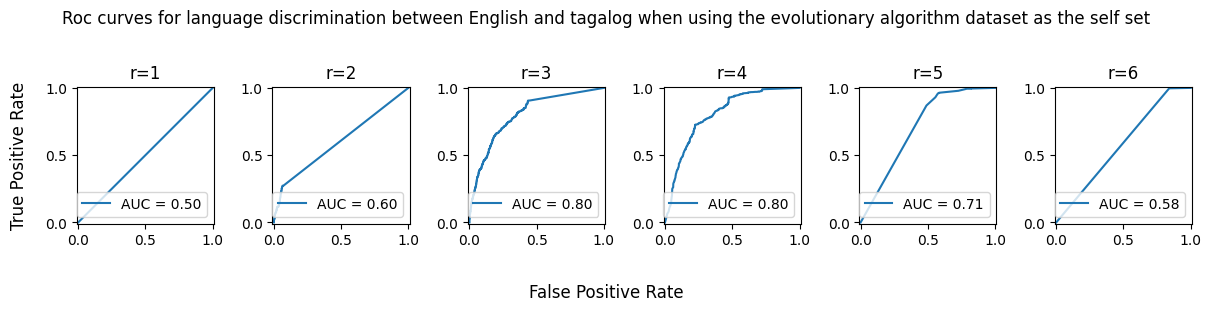
\includegraphics[width=\linewidth]{images/english_tagalog_ea.png}
        \label{fig:eng_mid_tag_ea}
    \end{subfigure}
        \\
    \begin{subfigure}[t]{\linewidth}
        \centering
        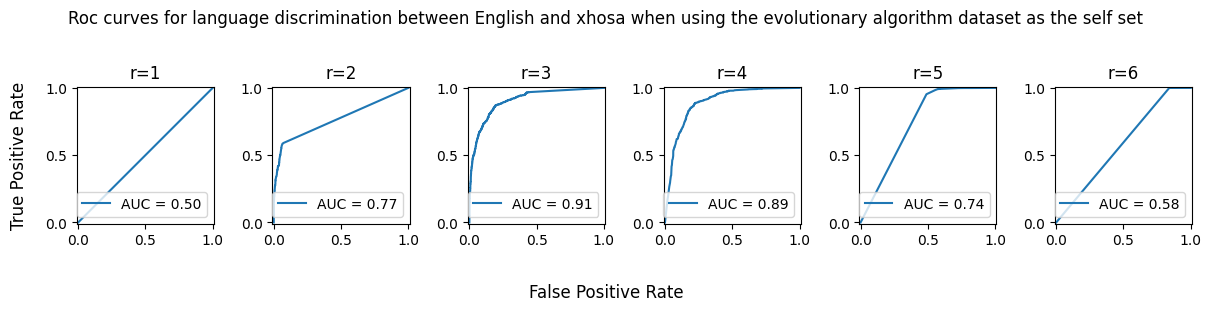
\includegraphics[width=\linewidth]{images/english_xhosa_ea.png}
        \label{fig:eng_xho_ea}
    \end{subfigure}
    
    \caption{ROC curves for language Discrimination between English and each other language, when using the evolutionary algorithm dataset for the self set}
    \label{fig:langs_ea}
\end{figure}

\begin{figure}[ht]
    \begin{subfigure}[t]{\linewidth}
        \centering
        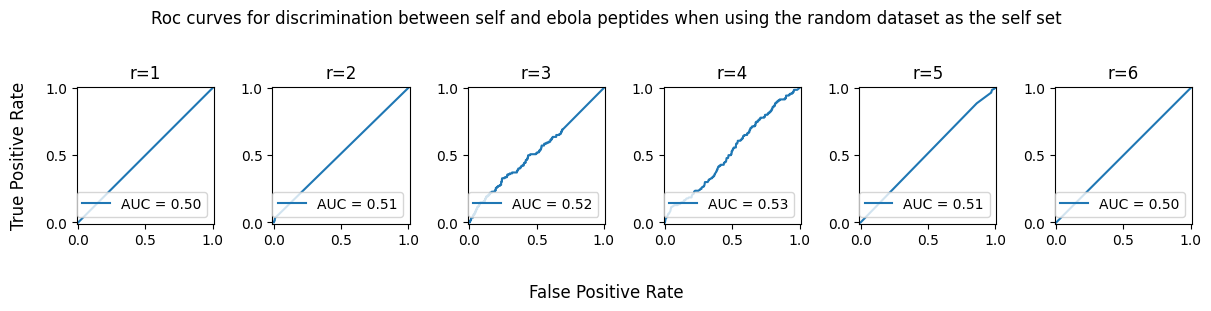
\includegraphics[width=\linewidth]{images/ebola_random.png}
        \label{fig:ebola_rnd}
    \end{subfigure}
    \\
    \begin{subfigure}[t]{\linewidth}
        \centering
        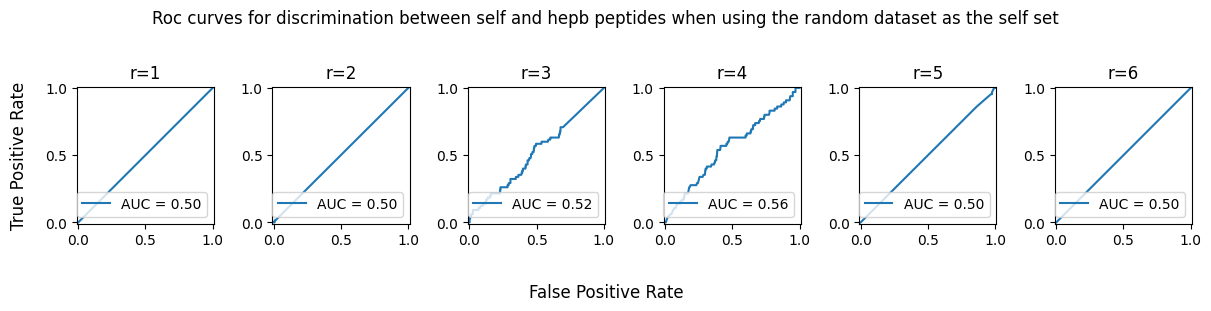
\includegraphics[width=\linewidth]{images/hepb_random.png}
        \label{fig:hepb_rnd}
    \end{subfigure}
        \\
    \begin{subfigure}[t]{\linewidth}
        \centering
        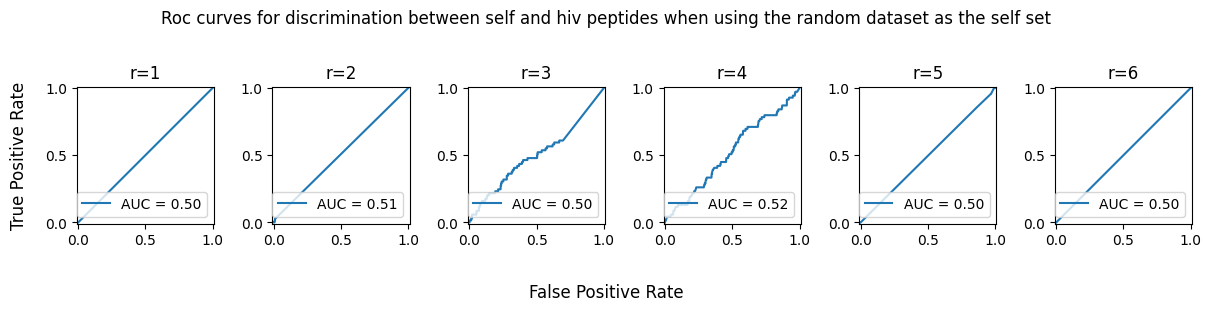
\includegraphics[width=\linewidth]{images/hiv_random.png}
        \label{fig:hiv_rnd}
    \end{subfigure}

    \caption{ROC curves for peptide detection between self and foreign, when using the random dataset for the self set}
    \label{fig:pept_rnd}
\end{figure}

\begin{figure}[ht]
    \begin{subfigure}[t]{\linewidth}
        \centering
        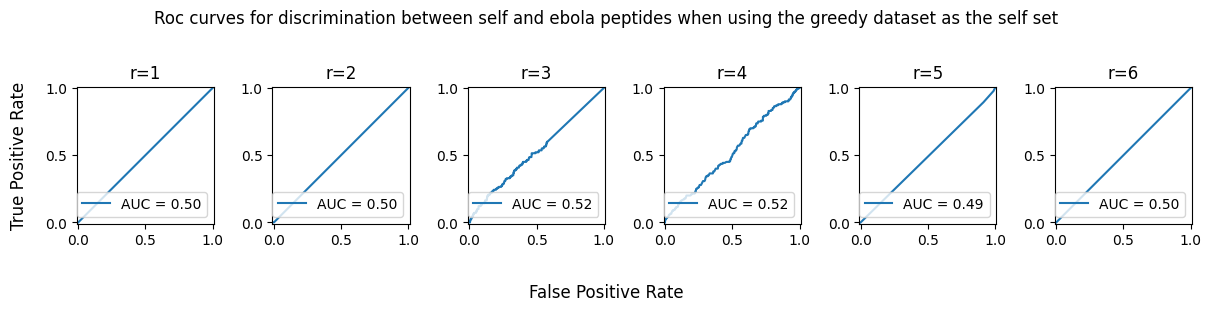
\includegraphics[width=\linewidth]{images/ebola_greedy.png}
        \label{fig:ebola_grd}
    \end{subfigure}
    \\
    \begin{subfigure}[t]{\linewidth}
        \centering
        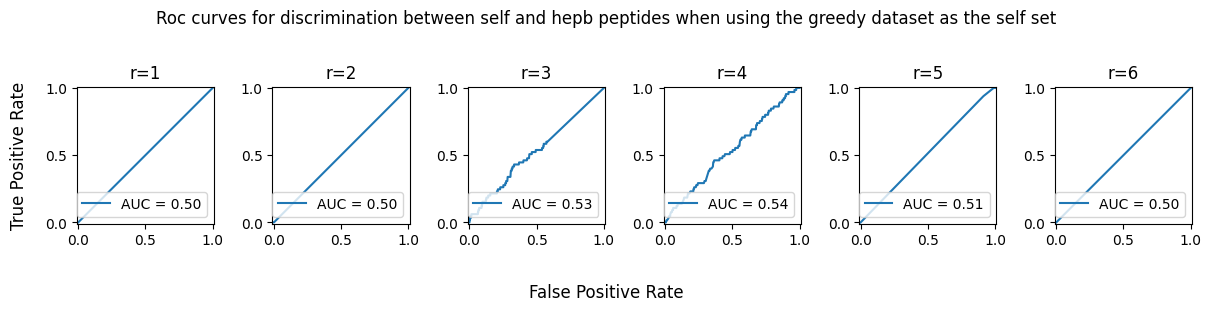
\includegraphics[width=\linewidth]{images/hepb_greedy.png}
        \label{fig:hepb_grd}
    \end{subfigure}
        \\
    \begin{subfigure}[t]{\linewidth}
        \centering
        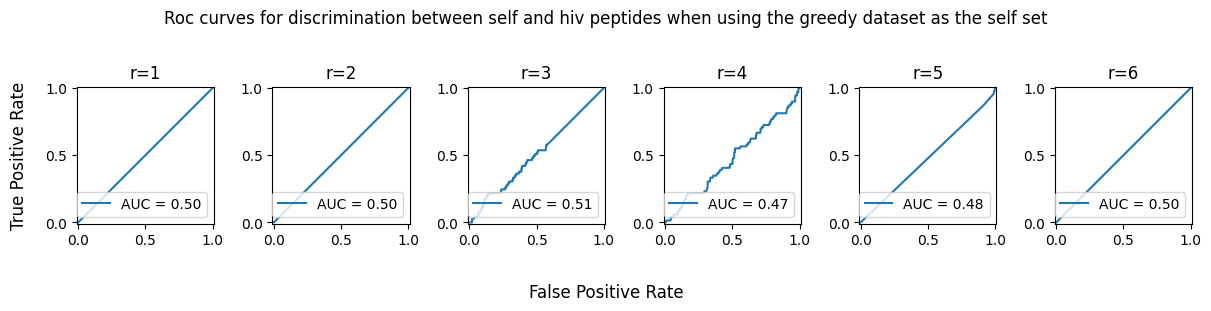
\includegraphics[width=\linewidth]{images/hiv_greedy.png}
        \label{fig:hiv_grd}
    \end{subfigure}

    \caption{ROC curves for peptide detection between self and foreign, when using the greedy dataset for the self set}
    \label{fig:pept_grd}
\end{figure}

\begin{figure}[ht]
    \begin{subfigure}[t]{\linewidth}
        \centering
        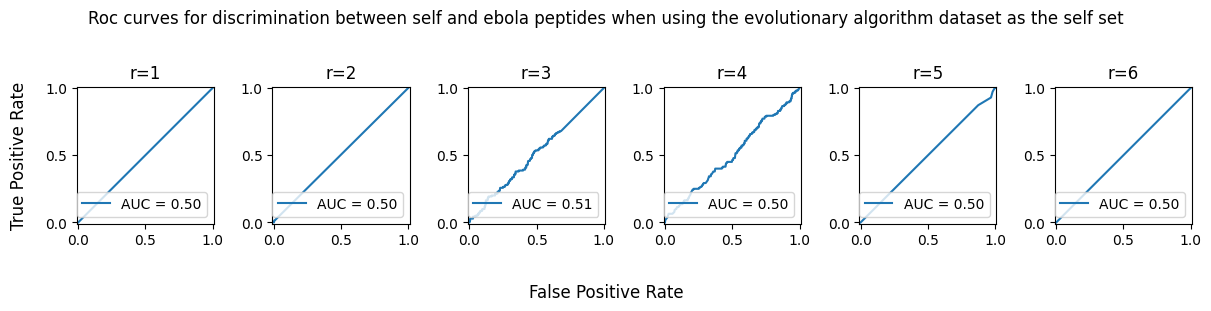
\includegraphics[width=\linewidth]{images/ebola_ea.png}
        \label{fig:ebola_ea}
    \end{subfigure}
    \\
    \begin{subfigure}[t]{\linewidth}
        \centering
        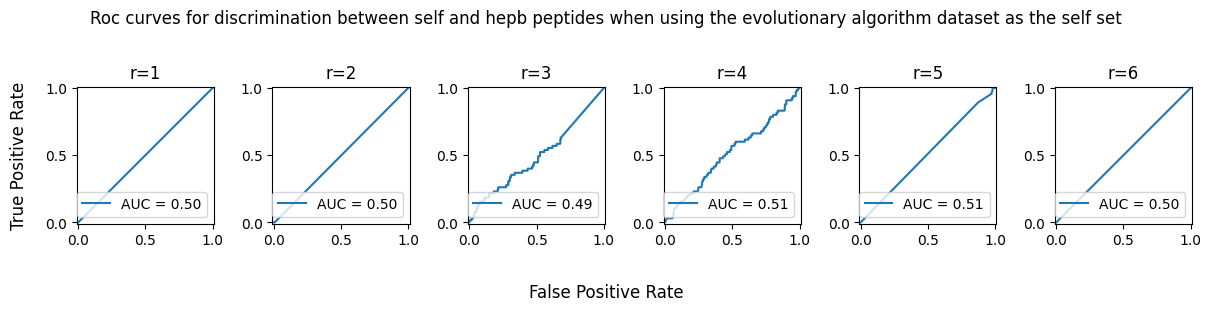
\includegraphics[width=\linewidth]{images/hepb_ea.png}
        \label{fig:hepb_ea}
    \end{subfigure}
        \\
    \begin{subfigure}[t]{\linewidth}
        \centering
        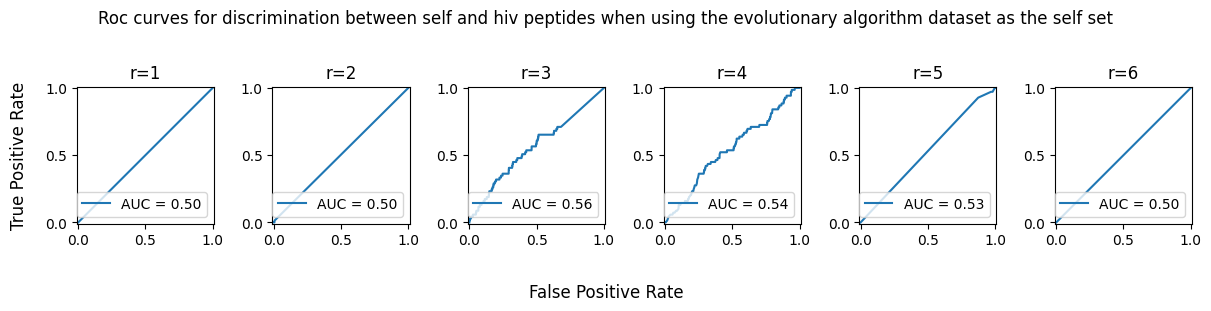
\includegraphics[width=\linewidth]{images/hiv_ea.png}
        \label{fig:hiv_ea}
    \end{subfigure}

    \caption{ROC curves for peptide detection between self and foreign, when using the evolutionary algorithm dataset for the self set}
    \label{fig:pept_ea}
\end{figure}

\end{document}